% Options for packages loaded elsewhere
\PassOptionsToPackage{unicode}{hyperref}
\PassOptionsToPackage{hyphens}{url}
\PassOptionsToPackage{dvipsnames,svgnames,x11names}{xcolor}
%
\documentclass[
  letterpaper,
  DIV=11,
  numbers=noendperiod]{scrreprt}

\usepackage{amsmath,amssymb}
\usepackage{lmodern}
\usepackage{iftex}
\ifPDFTeX
  \usepackage[T1]{fontenc}
  \usepackage[utf8]{inputenc}
  \usepackage{textcomp} % provide euro and other symbols
\else % if luatex or xetex
  \usepackage{unicode-math}
  \defaultfontfeatures{Scale=MatchLowercase}
  \defaultfontfeatures[\rmfamily]{Ligatures=TeX,Scale=1}
\fi
% Use upquote if available, for straight quotes in verbatim environments
\IfFileExists{upquote.sty}{\usepackage{upquote}}{}
\IfFileExists{microtype.sty}{% use microtype if available
  \usepackage[]{microtype}
  \UseMicrotypeSet[protrusion]{basicmath} % disable protrusion for tt fonts
}{}
\makeatletter
\@ifundefined{KOMAClassName}{% if non-KOMA class
  \IfFileExists{parskip.sty}{%
    \usepackage{parskip}
  }{% else
    \setlength{\parindent}{0pt}
    \setlength{\parskip}{6pt plus 2pt minus 1pt}}
}{% if KOMA class
  \KOMAoptions{parskip=half}}
\makeatother
\usepackage{xcolor}
\setlength{\emergencystretch}{3em} % prevent overfull lines
\setcounter{secnumdepth}{5}
% Make \paragraph and \subparagraph free-standing
\ifx\paragraph\undefined\else
  \let\oldparagraph\paragraph
  \renewcommand{\paragraph}[1]{\oldparagraph{#1}\mbox{}}
\fi
\ifx\subparagraph\undefined\else
  \let\oldsubparagraph\subparagraph
  \renewcommand{\subparagraph}[1]{\oldsubparagraph{#1}\mbox{}}
\fi

\usepackage{color}
\usepackage{fancyvrb}
\newcommand{\VerbBar}{|}
\newcommand{\VERB}{\Verb[commandchars=\\\{\}]}
\DefineVerbatimEnvironment{Highlighting}{Verbatim}{commandchars=\\\{\}}
% Add ',fontsize=\small' for more characters per line
\usepackage{framed}
\definecolor{shadecolor}{RGB}{241,243,245}
\newenvironment{Shaded}{\begin{snugshade}}{\end{snugshade}}
\newcommand{\AlertTok}[1]{\textcolor[rgb]{0.68,0.00,0.00}{#1}}
\newcommand{\AnnotationTok}[1]{\textcolor[rgb]{0.37,0.37,0.37}{#1}}
\newcommand{\AttributeTok}[1]{\textcolor[rgb]{0.40,0.45,0.13}{#1}}
\newcommand{\BaseNTok}[1]{\textcolor[rgb]{0.68,0.00,0.00}{#1}}
\newcommand{\BuiltInTok}[1]{\textcolor[rgb]{0.00,0.23,0.31}{#1}}
\newcommand{\CharTok}[1]{\textcolor[rgb]{0.13,0.47,0.30}{#1}}
\newcommand{\CommentTok}[1]{\textcolor[rgb]{0.37,0.37,0.37}{#1}}
\newcommand{\CommentVarTok}[1]{\textcolor[rgb]{0.37,0.37,0.37}{\textit{#1}}}
\newcommand{\ConstantTok}[1]{\textcolor[rgb]{0.56,0.35,0.01}{#1}}
\newcommand{\ControlFlowTok}[1]{\textcolor[rgb]{0.00,0.23,0.31}{#1}}
\newcommand{\DataTypeTok}[1]{\textcolor[rgb]{0.68,0.00,0.00}{#1}}
\newcommand{\DecValTok}[1]{\textcolor[rgb]{0.68,0.00,0.00}{#1}}
\newcommand{\DocumentationTok}[1]{\textcolor[rgb]{0.37,0.37,0.37}{\textit{#1}}}
\newcommand{\ErrorTok}[1]{\textcolor[rgb]{0.68,0.00,0.00}{#1}}
\newcommand{\ExtensionTok}[1]{\textcolor[rgb]{0.00,0.23,0.31}{#1}}
\newcommand{\FloatTok}[1]{\textcolor[rgb]{0.68,0.00,0.00}{#1}}
\newcommand{\FunctionTok}[1]{\textcolor[rgb]{0.28,0.35,0.67}{#1}}
\newcommand{\ImportTok}[1]{\textcolor[rgb]{0.00,0.46,0.62}{#1}}
\newcommand{\InformationTok}[1]{\textcolor[rgb]{0.37,0.37,0.37}{#1}}
\newcommand{\KeywordTok}[1]{\textcolor[rgb]{0.00,0.23,0.31}{#1}}
\newcommand{\NormalTok}[1]{\textcolor[rgb]{0.00,0.23,0.31}{#1}}
\newcommand{\OperatorTok}[1]{\textcolor[rgb]{0.37,0.37,0.37}{#1}}
\newcommand{\OtherTok}[1]{\textcolor[rgb]{0.00,0.23,0.31}{#1}}
\newcommand{\PreprocessorTok}[1]{\textcolor[rgb]{0.68,0.00,0.00}{#1}}
\newcommand{\RegionMarkerTok}[1]{\textcolor[rgb]{0.00,0.23,0.31}{#1}}
\newcommand{\SpecialCharTok}[1]{\textcolor[rgb]{0.37,0.37,0.37}{#1}}
\newcommand{\SpecialStringTok}[1]{\textcolor[rgb]{0.13,0.47,0.30}{#1}}
\newcommand{\StringTok}[1]{\textcolor[rgb]{0.13,0.47,0.30}{#1}}
\newcommand{\VariableTok}[1]{\textcolor[rgb]{0.07,0.07,0.07}{#1}}
\newcommand{\VerbatimStringTok}[1]{\textcolor[rgb]{0.13,0.47,0.30}{#1}}
\newcommand{\WarningTok}[1]{\textcolor[rgb]{0.37,0.37,0.37}{\textit{#1}}}

\providecommand{\tightlist}{%
  \setlength{\itemsep}{0pt}\setlength{\parskip}{0pt}}\usepackage{longtable,booktabs,array}
\usepackage{calc} % for calculating minipage widths
% Correct order of tables after \paragraph or \subparagraph
\usepackage{etoolbox}
\makeatletter
\patchcmd\longtable{\par}{\if@noskipsec\mbox{}\fi\par}{}{}
\makeatother
% Allow footnotes in longtable head/foot
\IfFileExists{footnotehyper.sty}{\usepackage{footnotehyper}}{\usepackage{footnote}}
\makesavenoteenv{longtable}
\usepackage{graphicx}
\makeatletter
\def\maxwidth{\ifdim\Gin@nat@width>\linewidth\linewidth\else\Gin@nat@width\fi}
\def\maxheight{\ifdim\Gin@nat@height>\textheight\textheight\else\Gin@nat@height\fi}
\makeatother
% Scale images if necessary, so that they will not overflow the page
% margins by default, and it is still possible to overwrite the defaults
% using explicit options in \includegraphics[width, height, ...]{}
\setkeys{Gin}{width=\maxwidth,height=\maxheight,keepaspectratio}
% Set default figure placement to htbp
\makeatletter
\def\fps@figure{htbp}
\makeatother
\newlength{\cslhangindent}
\setlength{\cslhangindent}{1.5em}
\newlength{\csllabelwidth}
\setlength{\csllabelwidth}{3em}
\newlength{\cslentryspacingunit} % times entry-spacing
\setlength{\cslentryspacingunit}{\parskip}
\newenvironment{CSLReferences}[2] % #1 hanging-ident, #2 entry spacing
 {% don't indent paragraphs
  \setlength{\parindent}{0pt}
  % turn on hanging indent if param 1 is 1
  \ifodd #1
  \let\oldpar\par
  \def\par{\hangindent=\cslhangindent\oldpar}
  \fi
  % set entry spacing
  \setlength{\parskip}{#2\cslentryspacingunit}
 }%
 {}
\usepackage{calc}
\newcommand{\CSLBlock}[1]{#1\hfill\break}
\newcommand{\CSLLeftMargin}[1]{\parbox[t]{\csllabelwidth}{#1}}
\newcommand{\CSLRightInline}[1]{\parbox[t]{\linewidth - \csllabelwidth}{#1}\break}
\newcommand{\CSLIndent}[1]{\hspace{\cslhangindent}#1}

\KOMAoption{captions}{tableheading}
\makeatletter
\makeatother
\makeatletter
\@ifpackageloaded{bookmark}{}{\usepackage{bookmark}}
\makeatother
\makeatletter
\@ifpackageloaded{caption}{}{\usepackage{caption}}
\AtBeginDocument{%
\ifdefined\contentsname
  \renewcommand*\contentsname{Table of contents}
\else
  \newcommand\contentsname{Table of contents}
\fi
\ifdefined\listfigurename
  \renewcommand*\listfigurename{List of Figures}
\else
  \newcommand\listfigurename{List of Figures}
\fi
\ifdefined\listtablename
  \renewcommand*\listtablename{List of Tables}
\else
  \newcommand\listtablename{List of Tables}
\fi
\ifdefined\figurename
  \renewcommand*\figurename{Figure}
\else
  \newcommand\figurename{Figure}
\fi
\ifdefined\tablename
  \renewcommand*\tablename{Table}
\else
  \newcommand\tablename{Table}
\fi
}
\@ifpackageloaded{float}{}{\usepackage{float}}
\floatstyle{ruled}
\@ifundefined{c@chapter}{\newfloat{codelisting}{h}{lop}}{\newfloat{codelisting}{h}{lop}[chapter]}
\floatname{codelisting}{Listing}
\newcommand*\listoflistings{\listof{codelisting}{List of Listings}}
\makeatother
\makeatletter
\@ifpackageloaded{caption}{}{\usepackage{caption}}
\@ifpackageloaded{subcaption}{}{\usepackage{subcaption}}
\makeatother
\makeatletter
\@ifpackageloaded{tcolorbox}{}{\usepackage[many]{tcolorbox}}
\makeatother
\makeatletter
\@ifundefined{shadecolor}{\definecolor{shadecolor}{rgb}{.97, .97, .97}}
\makeatother
\makeatletter
\makeatother
\ifLuaTeX
  \usepackage{selnolig}  % disable illegal ligatures
\fi
\IfFileExists{bookmark.sty}{\usepackage{bookmark}}{\usepackage{hyperref}}
\IfFileExists{xurl.sty}{\usepackage{xurl}}{} % add URL line breaks if available
\urlstyle{same} % disable monospaced font for URLs
\hypersetup{
  pdftitle={Doing Bayesian Data Analysis in Julia using Turing.jl},
  pdfauthor={Kianté Fernandez},
  colorlinks=true,
  linkcolor={blue},
  filecolor={Maroon},
  citecolor={Blue},
  urlcolor={Blue},
  pdfcreator={LaTeX via pandoc}}

\title{Doing Bayesian Data Analysis in Julia using Turing.jl}
\author{Kianté Fernandez}
\date{8/25/2022}

\begin{document}
\maketitle
\ifdefined\Shaded\renewenvironment{Shaded}{\begin{tcolorbox}[interior hidden, breakable, boxrule=0pt, frame hidden, borderline west={3pt}{0pt}{shadecolor}, enhanced, sharp corners]}{\end{tcolorbox}}\fi

\renewcommand*\contentsname{Table of contents}
{
\hypersetup{linkcolor=}
\setcounter{tocdepth}{2}
\tableofcontents
}
\bookmarksetup{startatroot}

\hypertarget{what-and-why}{%
\chapter*{What and why}\label{what-and-why}}
\addcontentsline{toc}{chapter}{What and why}

Kruschke began his text with, ``This book explains how to actually do
Bayesian data analysis, by real people (like you), for realistic data
(like yours).'' In the same way, this project is designed to help those
real people do Bayesian data analysis. My contribution is converting
Kruschke's JAGS and Stan code for use in another probabilistic
programming framework,\texttt{Turing.jl}, which makes it easier to fit
Bayesian regression models in Julia (Ge, Xu, and Ghahramani (2018))
using a number of samplers. I also prefer plotting and data wrangling
with the packages from \texttt{Plots.jl}(Bezanson et al. (2017)). So
we'll be using those methods, too.

This ebook is not meant to stand alone. It's a supplement to the second
edition of Kruschke (2015) Doing Bayesian data analysis: A tutorial with
R, JAGS, and Stan. Please give the source material some love.

\hypertarget{julia-setup}{%
\section*{Julia setup}\label{julia-setup}}
\addcontentsline{toc}{section}{Julia setup}

To follow along with this guide, you'll need some software. Download and
install Julia by following the instructions at
\href{https://julialang.org/downloads/}{https://julialang.org/downloads/.}
The
\href{https://docs.julialang.org/en/v1/manual/getting-started/}{Getting
Started page} has in depth instructions that can help.

\hypertarget{version-0.0.1.}{%
\section*{Version 0.0.1.}\label{version-0.0.1.}}
\addcontentsline{toc}{section}{Version 0.0.1.}

I am just starting this project. I plan to have a complete draft
including material from all the chapters in Kruschke's text by January
2023

\bookmarksetup{startatroot}

\hypertarget{whats-in-this-book-read-this-first}{%
\chapter{What's in This Book (Read This
First!)}\label{whats-in-this-book-read-this-first}}

\hypertarget{gimme-feedback-be-polite}{%
\section{Gimme feedback (be polite)}\label{gimme-feedback-be-polite}}

I am not a statistician and have no formal computer science background.
I am in the process of learning the Julia programming language (part of
the goal of this project!). I am currently a Ph.D.~student in
psychology. I have been mostly an R and MATLAB user and started learning
Bayesian statistics around 2019. My code will likely be ``bad'' as I get
the hang of things. I have much to learn from the Julia community and
thus encourage folk to reach out with suggestions on how to improve my
code. If you'd like to learn more about me, you can find my website at
\href{https://www.kiantefernandez.com/}{https://www.kiantefernandez.com/.}

\hypertarget{thank-you}{%
\section{Thank you!}\label{thank-you}}

A. Solomon Kurz really inspired this project. He has published multiple
accessible introductory content on applied Bayesian analysis,
complementing many of the books that taught me Bayesian statistics. I
benefitted greatly from his free content. Go find him at:
\url{https://solomonkurz.netlify.com.}

\bookmarksetup{startatroot}

\hypertarget{introduction-credibility-models-and-parameters}{%
\chapter{Introduction: Credibility, Models, and
Parameters}\label{introduction-credibility-models-and-parameters}}

\hypertarget{bayesian-inference-is-reallocation-of-credibility-across-possibilities}{%
\section{Bayesian inference is reallocation of credibility across
possibilities}\label{bayesian-inference-is-reallocation-of-credibility-across-possibilities}}

To make Figure 2.1 we need data. We will create some synthetic data and
store it in using \texttt{DataFrames.jl}

\begin{Shaded}
\begin{Highlighting}[]
\ImportTok{using} \BuiltInTok{DataFrames}

\KeywordTok{function} \FunctionTok{expand\_grid}\NormalTok{(; iters}\OperatorTok{...}\NormalTok{)}
\NormalTok{    var\_names }\OperatorTok{=} \FunctionTok{collect}\NormalTok{(}\FunctionTok{keys}\NormalTok{(iters))}
\NormalTok{    var\_itr }\OperatorTok{=}\NormalTok{ [}\FloatTok{1}\OperatorTok{:}\FunctionTok{length}\NormalTok{(x) for x }\KeywordTok{in}\NormalTok{ iters.data]}
\NormalTok{    var\_ix }\OperatorTok{=} \FunctionTok{vcat}\NormalTok{([}\FunctionTok{collect}\NormalTok{(x)}\CharTok{\textquotesingle{} for x in Iterators.product(var\_itr...)]...)}
\NormalTok{    out }\OperatorTok{=} \FunctionTok{DataFrame}\NormalTok{()}
\NormalTok{    for i }\OperatorTok{=} \FloatTok{1}\OperatorTok{:}\FunctionTok{length}\NormalTok{(var\_names)}
\NormalTok{        out[}\OperatorTok{:}\NormalTok{,var\_names[i]] }\OperatorTok{=} \FunctionTok{collect}\NormalTok{(iters[i])[var\_ix[}\OperatorTok{:}\NormalTok{,i]]}
    \KeywordTok{end}
\NormalTok{    return out}
\KeywordTok{end}

\NormalTok{d }\OperatorTok{=} \FunctionTok{expand\_grid}\NormalTok{(iteration}\OperatorTok{=}\FloatTok{1}\OperatorTok{:}\FloatTok{3}\NormalTok{, Possibilities}\OperatorTok{=}\NormalTok{[}\StringTok{"a"}\NormalTok{, }\StringTok{"b"}\NormalTok{,}\StringTok{"c"}\NormalTok{, }\StringTok{"d"}\NormalTok{], stage }\OperatorTok{=}\NormalTok{ [}\StringTok{"a"}\NormalTok{, }\StringTok{"b"}\NormalTok{])}

\NormalTok{d2 }\OperatorTok{=}\FunctionTok{DataFrame}\NormalTok{(Credibility }\OperatorTok{=}\NormalTok{[}\FunctionTok{fill}\NormalTok{(}\FloatTok{.25}\NormalTok{,}\FloatTok{4}\NormalTok{); }\FloatTok{0}\NormalTok{; }\FunctionTok{fill}\NormalTok{(}\FloatTok{1}\OperatorTok{/}\FloatTok{3}\NormalTok{,}\FloatTok{3}\NormalTok{); }\FloatTok{0}\NormalTok{; }\FunctionTok{fill}\NormalTok{(}\FloatTok{1}\OperatorTok{/}\FloatTok{3}\NormalTok{,}\FloatTok{3}\NormalTok{);}\FloatTok{0}\NormalTok{;}\FloatTok{.5}\NormalTok{;}\FloatTok{0}\NormalTok{;}\FloatTok{0.5}\NormalTok{;}\FloatTok{0}\NormalTok{;}\FloatTok{.5}\NormalTok{;}\FloatTok{0}\NormalTok{;}\FloatTok{0.5}\NormalTok{;}\FunctionTok{fill}\NormalTok{(}\FloatTok{0}\NormalTok{,}\FloatTok{3}\NormalTok{);}\FloatTok{1}\NormalTok{])}

\FunctionTok{sort!}\NormalTok{(d, [}\OperatorTok{:}\NormalTok{iteration])}
\NormalTok{d.Credibility }\OperatorTok{=}\NormalTok{ d2.Credibility}
\end{Highlighting}
\end{Shaded}

\begin{verbatim}
┌ Warning: use values(kwargs) and keys(kwargs) instead of kwargs.data and kwargs.itr
│   caller = expand_grid(; iters::Base.Pairs{Symbol, AbstractVector, Tuple{Symbol, Symbol, Symbol}, NamedTuple{(:iteration, :Possibilities, :stage), Tuple{UnitRange{Int64}, Vector{String}, Vector{String}}}}) at In[2]:5
└ @ Main ./In[2]:5
\end{verbatim}

\begin{verbatim}
24-element Vector{Float64}:
 0.25
 0.25
 0.25
 0.25
 0.0
 0.3333333333333333
 0.3333333333333333
 0.3333333333333333
 0.0
 0.3333333333333333
 0.3333333333333333
 0.3333333333333333
 0.0
 0.5
 0.0
 0.5
 0.0
 0.5
 0.0
 0.5
 0.0
 0.0
 0.0
 1.0
\end{verbatim}

Here we are defining a function that creates combinations and then I
just bind that we the Credibility values we will use for plotting.

We can take a look at the top few rows of the data with the
\texttt{first()} function.

\begin{Shaded}
\begin{Highlighting}[]
\FunctionTok{first}\NormalTok{(d,}\FloatTok{5}\NormalTok{)}
\end{Highlighting}
\end{Shaded}

\begin{tabular}{r|cccc}
    & iteration & Possibilities & stage & Credibility\\
    \hline
    & Int64 & String & String & Float64\\
    \hline
    1 & 1 & a & a & 0.25 \\
    2 & 1 & b & a & 0.25 \\
    3 & 1 & c & a & 0.25 \\
    4 & 1 & d & a & 0.25 \\
    5 & 1 & a & b & 0.0 \\
\end{tabular}

Now lets plot our version of Figure 2.1:

\begin{Shaded}
\begin{Highlighting}[]
\ImportTok{using} \BuiltInTok{Plots}
\ImportTok{using} \BuiltInTok{VegaLite}

\CommentTok{\#bar(d.Possibilities, d.Credibility, layout = 6)}

\NormalTok{d }\OperatorTok{|\textgreater{}}
\PreprocessorTok{@vlplot}\NormalTok{(}
  \OperatorTok{:}\NormalTok{bar,}
\NormalTok{  color}\OperatorTok{=:}\NormalTok{green,}
\NormalTok{  column }\OperatorTok{=}\NormalTok{ \{}\StringTok{"iteration"}\NormalTok{,axis}\OperatorTok{=}\NormalTok{\{title}\OperatorTok{=}\StringTok{""}\NormalTok{\}\},}
\NormalTok{  row }\OperatorTok{=}\NormalTok{ \{}\StringTok{"stage:o"}\NormalTok{, sort }\OperatorTok{=} \StringTok{"{-}stage"}\NormalTok{, axis}\OperatorTok{=}\NormalTok{\{title}\OperatorTok{=}\StringTok{""}\NormalTok{\}\},}
\NormalTok{  x}\OperatorTok{=}\NormalTok{\{}\StringTok{"Possibilities:n"}\NormalTok{, title}\OperatorTok{=}\StringTok{"Possibilities"}\NormalTok{\},}
\NormalTok{  color}\OperatorTok{=}\NormalTok{\{}\StringTok{"Possibilities:n"}\NormalTok{, scale}\OperatorTok{=}\NormalTok{\{range}\OperatorTok{=}\NormalTok{[}\StringTok{"\#89b8f5"}\NormalTok{]\}, axis}\OperatorTok{=}\NormalTok{\{title}\OperatorTok{=}\StringTok{""}\NormalTok{\}, legend }\OperatorTok{=} \StringTok{""}\NormalTok{\},}
\NormalTok{  y}\OperatorTok{=}\NormalTok{\{}\StringTok{"Credibility"}\NormalTok{, axis}\OperatorTok{=}\NormalTok{\{title}\OperatorTok{=}\StringTok{"Credibility"}\NormalTok{, grid}\OperatorTok{=}\ConstantTok{false}\NormalTok{\}\},}
\NormalTok{  height }\OperatorTok{=} \FloatTok{250}\NormalTok{)}
\end{Highlighting}
\end{Shaded}

\begin{figure}[H]

{\centering 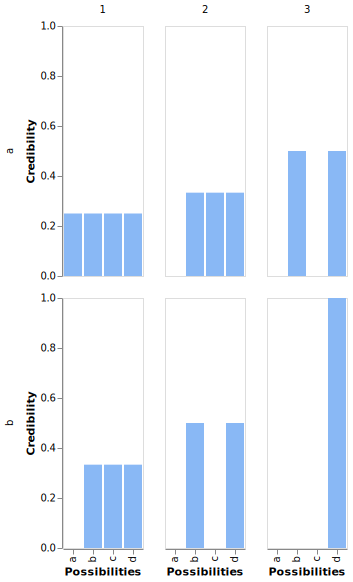
\includegraphics{./introduction-credibility-models-and-parameters_files/figure-pdf/cell-4-output-1.svg}

}

\end{figure}

\begin{verbatim}
WARN column encoding should be discrete (ordinal / nominal / binned).
WARN column encoding should be discrete (ordinal / nominal / binned).
WARN column encoding should be discrete (ordinal / nominal / binned).
\end{verbatim}

\bookmarksetup{startatroot}

\hypertarget{the-julia-programming-language}{%
\chapter{The Julia programming
language}\label{the-julia-programming-language}}

\bookmarksetup{startatroot}

\hypertarget{what-is-this-stuff-called-probability}{%
\chapter{What is This Stuff Called
Probability?}\label{what-is-this-stuff-called-probability}}

\bookmarksetup{startatroot}

\hypertarget{bayes-rule}{%
\chapter{Bayes' Rule}\label{bayes-rule}}

\bookmarksetup{startatroot}

\hypertarget{inferring-a-binomial-probability-via-exact-mathematical-analysis}{%
\chapter{Inferring a Binomial Probability via Exact Mathematical
Analysis}\label{inferring-a-binomial-probability-via-exact-mathematical-analysis}}

\bookmarksetup{startatroot}

\hypertarget{markov-chain-monte-carlo}{%
\chapter{Markov Chain Monte Carlo}\label{markov-chain-monte-carlo}}

\bookmarksetup{startatroot}

\hypertarget{turing.jl}{%
\chapter{Turing.jl}\label{turing.jl}}

\bookmarksetup{startatroot}

\hypertarget{hierarchical-models}{%
\chapter{Hierarchical Models}\label{hierarchical-models}}

\bookmarksetup{startatroot}

\hypertarget{model-comparison-and-hierarchical-modeling}{%
\chapter{Model Comparison and Hierarchical
Modeling}\label{model-comparison-and-hierarchical-modeling}}

\bookmarksetup{startatroot}

\hypertarget{null-hypothesis-significance-testing}{%
\chapter{Null Hypothesis Significance
Testing}\label{null-hypothesis-significance-testing}}

\bookmarksetup{startatroot}

\hypertarget{bayesian-approaches-to-testing-a-point-null-hypothesis}{%
\chapter{Bayesian Approaches to Testing a Point (``Null'')
Hypothesis}\label{bayesian-approaches-to-testing-a-point-null-hypothesis}}

\bookmarksetup{startatroot}

\hypertarget{goals-power-and-sample-size}{%
\chapter{Goals, Power, and Sample
Size}\label{goals-power-and-sample-size}}

\bookmarksetup{startatroot}

\hypertarget{overview-of-the-generalized-linear-model}{%
\chapter{Overview of the Generalized Linear
Model}\label{overview-of-the-generalized-linear-model}}

\bookmarksetup{startatroot}

\hypertarget{metric-predicted-variable-on-one-or-two-groups}{%
\chapter{Metric-Predicted Variable on One or Two
Groups}\label{metric-predicted-variable-on-one-or-two-groups}}

\bookmarksetup{startatroot}

\hypertarget{metric-predicted-variable-with-one-metric-predictor}{%
\chapter{Metric Predicted Variable with One Metric
Predictor}\label{metric-predicted-variable-with-one-metric-predictor}}

\bookmarksetup{startatroot}

\hypertarget{metric-predicted-variable-with-multiple-metric-predictors}{%
\chapter{Metric Predicted Variable with Multiple Metric
Predictors}\label{metric-predicted-variable-with-multiple-metric-predictors}}

\bookmarksetup{startatroot}

\hypertarget{metric-predicted-variable-with-one-nominal-predictor}{%
\chapter{Metric Predicted Variable with One Nominal
Predictor}\label{metric-predicted-variable-with-one-nominal-predictor}}

\bookmarksetup{startatroot}

\hypertarget{metric-predicted-variable-with-multiple-nominal-predictors}{%
\chapter{Metric Predicted Variable with Multiple Nominal
Predictors}\label{metric-predicted-variable-with-multiple-nominal-predictors}}

\bookmarksetup{startatroot}

\hypertarget{dichotomous-predicted-variable}{%
\chapter{Dichotomous Predicted
Variable}\label{dichotomous-predicted-variable}}

\bookmarksetup{startatroot}

\hypertarget{nominal-predicted-variable}{%
\chapter{Nominal Predicted Variable}\label{nominal-predicted-variable}}

\bookmarksetup{startatroot}

\hypertarget{ordinal-predicted-variable}{%
\chapter{Ordinal Predicted Variable}\label{ordinal-predicted-variable}}

\bookmarksetup{startatroot}

\hypertarget{count-predicted-variable}{%
\chapter{Count Predicted Variable}\label{count-predicted-variable}}

\bookmarksetup{startatroot}

\hypertarget{tools-in-the-trunk}{%
\chapter{Tools in the Trunk}\label{tools-in-the-trunk}}

\bookmarksetup{startatroot}

\hypertarget{references}{%
\chapter*{References}\label{references}}
\addcontentsline{toc}{chapter}{References}

\hypertarget{refs}{}
\begin{CSLReferences}{1}{0}
\leavevmode\vadjust pre{\hypertarget{ref-bezanson2017julia}{}}%
Bezanson, Jeff, Alan Edelman, Stefan Karpinski, and Viral B Shah. 2017.
{``Julia: A Fresh Approach to Numerical Computing.''} \emph{SIAM Review}
59 (1): 65--98. \url{https://doi.org/10.1137/141000671}.

\leavevmode\vadjust pre{\hypertarget{ref-ge2018t}{}}%
Ge, Hong, Kai Xu, and Zoubin Ghahramani. 2018. {``Turing: A Language for
Flexible Probabilistic Inference.''} In \emph{International Conference
on Artificial Intelligence and Statistics, {AISTATS} 2018, 9-11 April
2018, Playa Blanca, Lanzarote, Canary Islands, Spain}, 1682--90.
\url{http://proceedings.mlr.press/v84/ge18b.html}.

\leavevmode\vadjust pre{\hypertarget{ref-kruschke2015doing}{}}%
Kruschke, John. 2015. \emph{Doing Bayesian Data Analysis (Second
Edition)}. Boston: Academic Press.

\end{CSLReferences}



\end{document}
